\documentclass{beamer}
\usepackage[utf8]{inputenc}
\usetheme{Singapore}
\usecolortheme{default}
\beamertemplatenavigationsymbolsempty
\usepackage{multicol}

\title[Dinamica molecolare] 
{Esercizio simulazione Monte-Carlo}

\author[Lorenzo Tasca]
{Lorenzo Tasca}

\institute[]
{
  Dipartimento di Fisica “Giuseppe Occhialini”\\
  Università degli Studi di Milano-Bicocca\\
}

\date[04/2024] 
{Aprile 2024 }



\begin{document}

\frame{\titlepage}

\begin{frame}
    \frametitle{Zero temperature MC, minimum energy configuration}

    $$N=25, E_{min}= -8\,eV$$

    \begin{figure}
        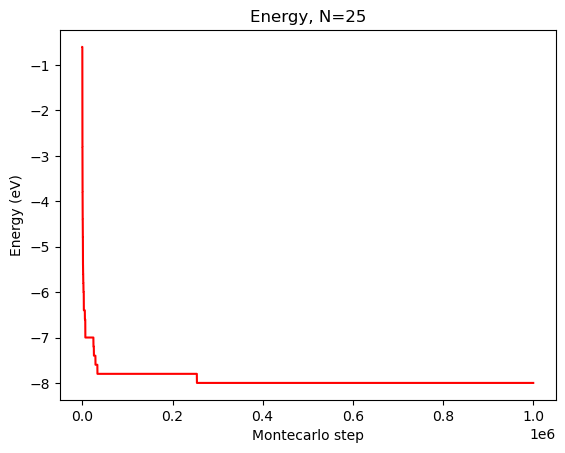
\includegraphics[width=0.7\textwidth]{images/energy25a.png}
    \end{figure}

\end{frame}

\begin{frame}
    \frametitle{Zero temperature MC, minimum energy configuration}

    $$N=25, E_{min}= -8\,eV$$

    \begin{figure}
        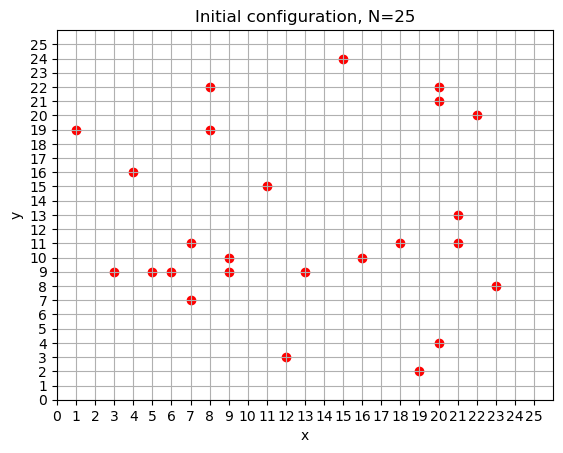
\includegraphics[width=0.7\textwidth]{images/initconf25a.png}
    \end{figure}

\end{frame}

\begin{frame}
    \frametitle{Zero temperature MC, minimum energy configuration}

    $$N=25, E_{min}= -8\,eV$$

    \begin{figure}
        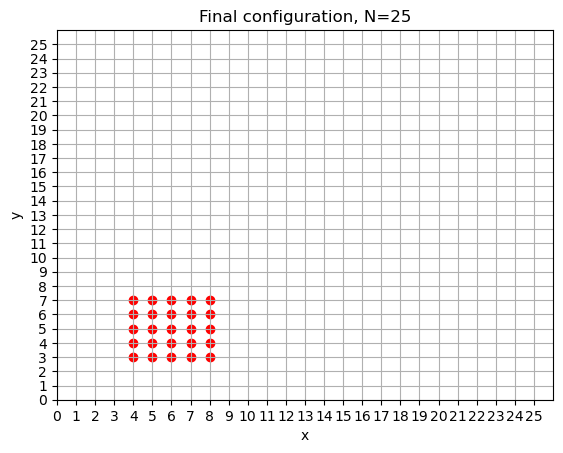
\includegraphics[width=0.7\textwidth]{images/finconf25a.png}
    \end{figure}

\end{frame}

\begin{frame}
    \frametitle{Zero temperature MC, minimum energy configuration}

    $$N=27, E_{min}= -8.6\,eV$$

    \begin{figure}
        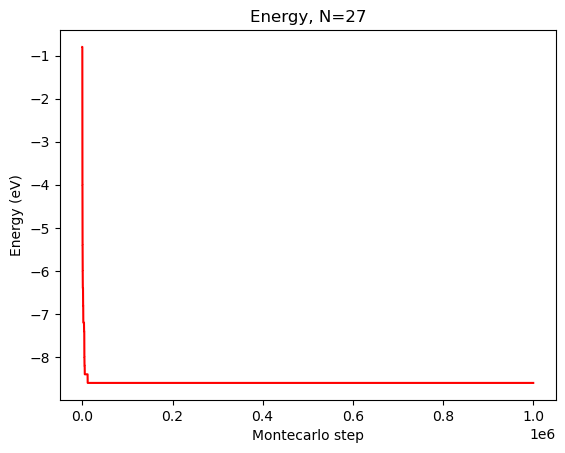
\includegraphics[width=0.7\textwidth]{images/energy27a.png}
    \end{figure}

\end{frame}

\begin{frame}
    \frametitle{Zero temperature MC, minimum energy configuration}

    $$N=27, E_{min}= -8.6\,eV$$

    \begin{figure}
        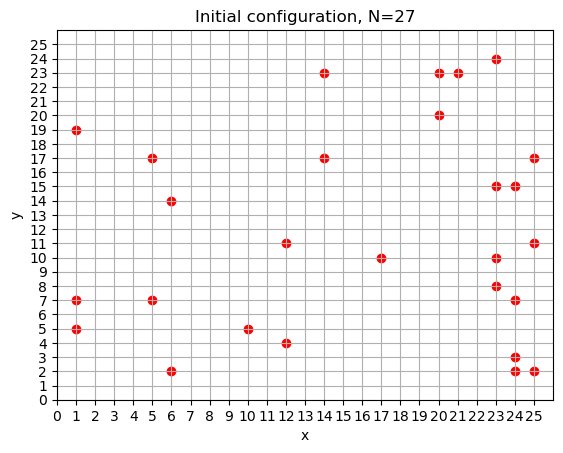
\includegraphics[width=0.7\textwidth]{images/initconf27a.png}
    \end{figure}

\end{frame}

\begin{frame}
    \frametitle{Zero temperature MC, minimum energy configuration}

    $$N=27, E_{min}= -8.6\,eV$$

    \begin{figure}
        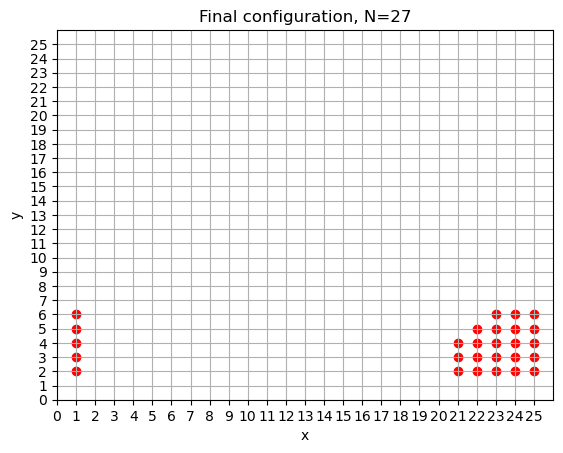
\includegraphics[width=0.7\textwidth]{images/finconf27a.png}
    \end{figure}

\end{frame}

\begin{frame}
    \frametitle{Zero temperature MC, minimum energy configuration}

    \centering Obtain minimum energy configuration for different values of $N$

    \begin{figure}
        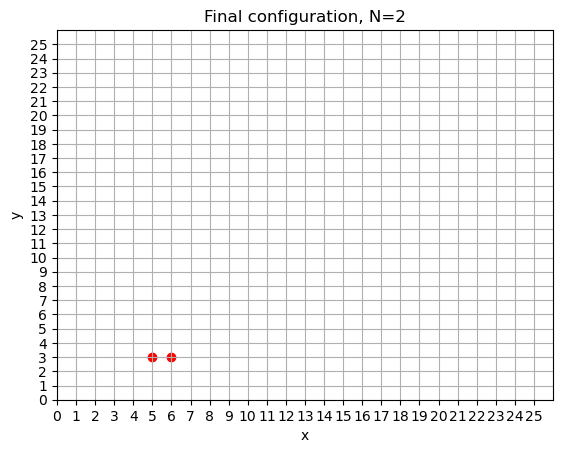
\includegraphics[width=0.7\textwidth]{images/finconf2b.png}
    \end{figure}

\end{frame}

\begin{frame}
    \frametitle{Zero temperature MC, minimum energy configuration}

    \centering Obtain minimum energy configuration for different values of $N$

    \begin{figure}
        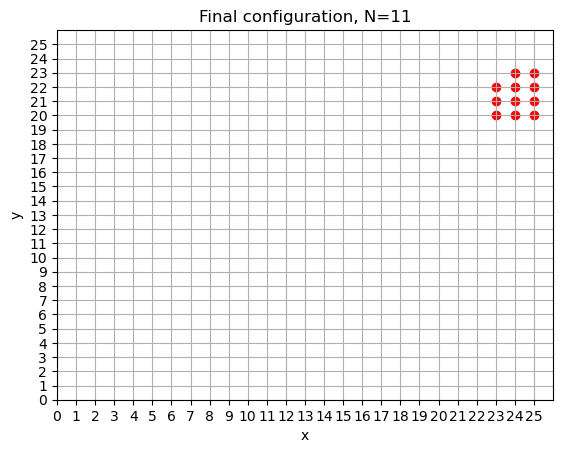
\includegraphics[width=0.7\textwidth]{images/finconf11b.png}
    \end{figure}

\end{frame}

\begin{frame}
    \frametitle{Zero temperature MC, minimum energy configuration}

    \centering Obtain minimum energy configuration for different values of $N$

    \begin{figure}
        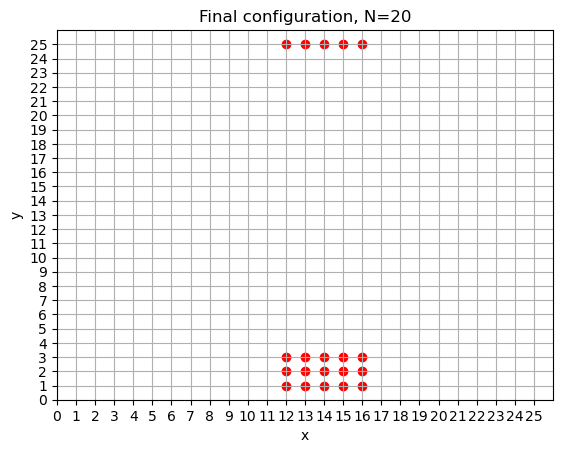
\includegraphics[width=0.7\textwidth]{images/finconf20b.png}
    \end{figure}

\end{frame}

\begin{frame}
    \frametitle{Zero temperature MC, energy variation with $N$}

    \begin{figure}
        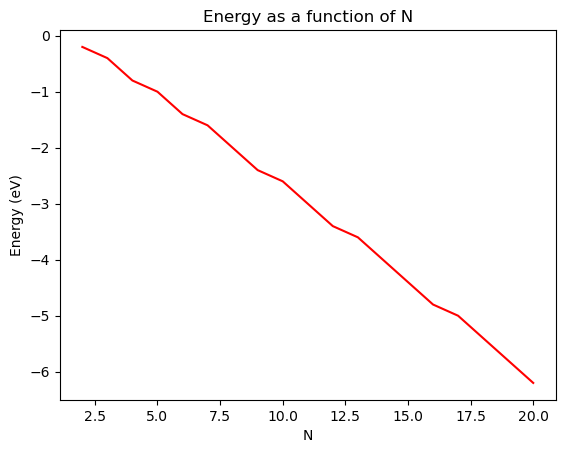
\includegraphics[width=0.7\textwidth]{images/energyb.png}
    \end{figure}

\end{frame}

\begin{frame}
    \frametitle{Zero temperature MC, $\mu$ variation with $N$}

    \begin{figure}
        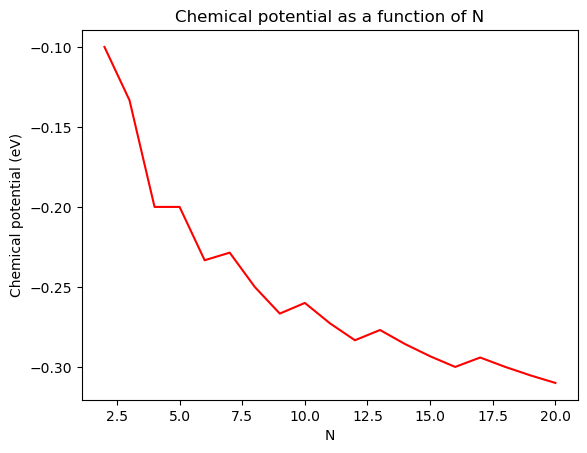
\includegraphics[width=0.7\textwidth]{images/mub.png}
    \end{figure}

\end{frame}

\begin{frame}
    \frametitle{Zero temperature MC, number of neighbours variation with $N$}

    \begin{figure}
        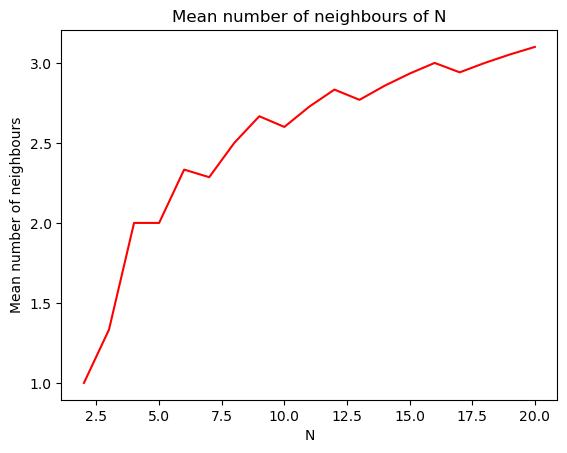
\includegraphics[width=0.7\textwidth]{images/nbrsb.png}
    \end{figure}

\end{frame}

\begin{frame}
    \frametitle{Finite temperature MC, $L=25$}

    $$T=4\,K$$

    \begin{figure}
        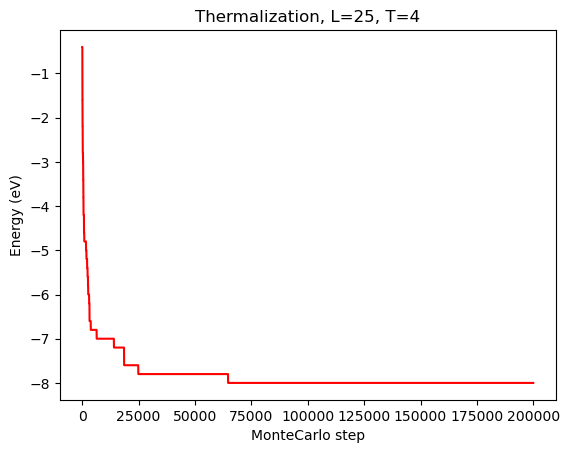
\includegraphics[width=0.7\textwidth]{images/cterm25T4.png}
    \end{figure}

\end{frame}

\begin{frame}
    \frametitle{Finite temperature MC, $L=25$}

    $$T=4\,K$$

    \begin{figure}
        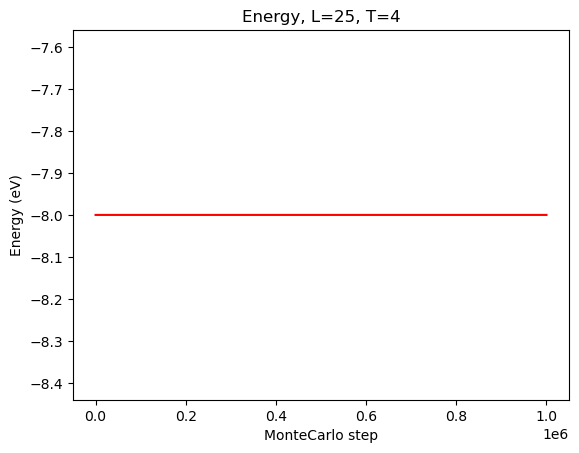
\includegraphics[width=0.7\textwidth]{images/cenergy25T4.png}
    \end{figure}

\end{frame}

\begin{frame}
    \frametitle{Finite temperature MC, $L=25$}

    $$T=604\,K$$

    \begin{figure}
        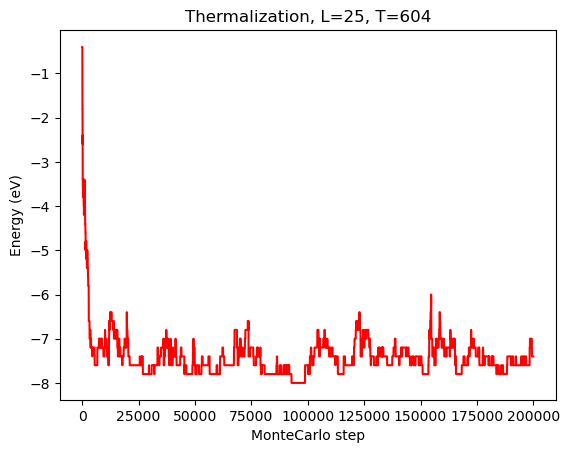
\includegraphics[width=0.7\textwidth]{images/cterm25T604.png}
    \end{figure}

\end{frame}

\begin{frame}
    \frametitle{Finite temperature MC, $L=25$}

    $$T=604\,K$$

    \begin{figure}
        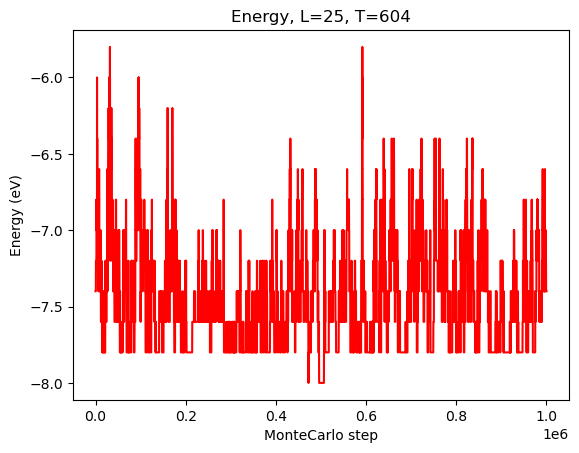
\includegraphics[width=0.7\textwidth]{images/cenergy25T604.png}
    \end{figure}

\end{frame}

\begin{frame}
    \frametitle{Finite temperature MC, $L=25$}

    $$T=1904\,K$$

    \begin{figure}
        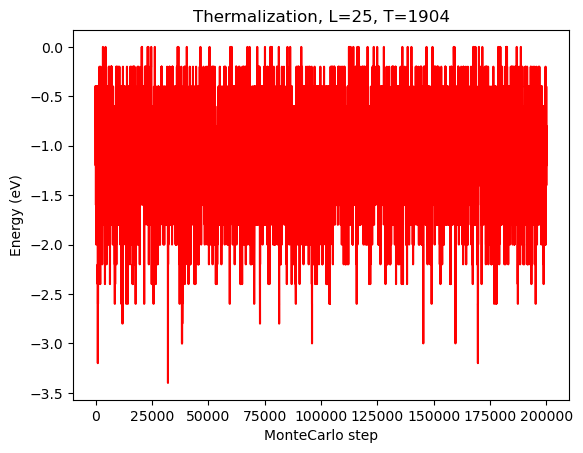
\includegraphics[width=0.7\textwidth]{images/cterm25T1904.png}
    \end{figure}

\end{frame}

\begin{frame}
    \frametitle{Finite temperature MC, $L=25$}

    $$T=1904\,K$$

    \begin{figure}
        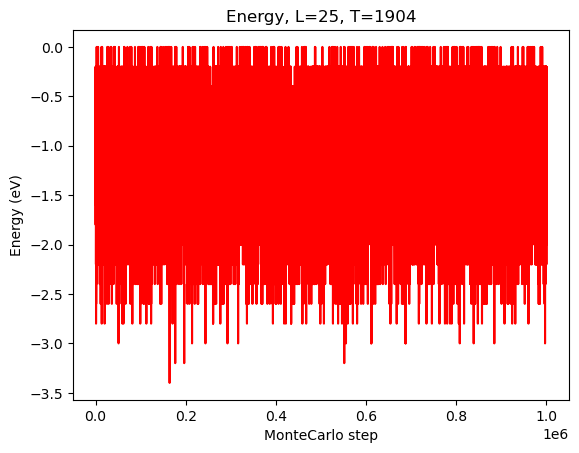
\includegraphics[width=0.7\textwidth]{images/cenergy25T1904.png}
    \end{figure}

\end{frame}

\begin{frame}
    \frametitle{Finite temperature MC, $L=15$}

    \centering Mean energy variation with temperature

    \begin{figure}
        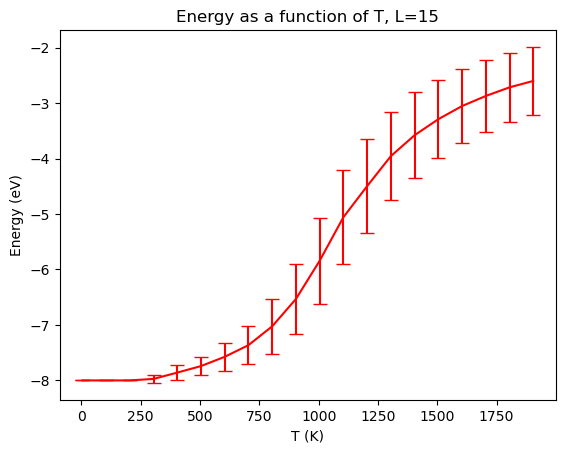
\includegraphics[width=0.7\textwidth]{images/cenergy15.png}
    \end{figure}

\end{frame}

\begin{frame}
    \frametitle{Finite temperature MC, $L=25$}

    \centering Mean energy variation with temperature

    \begin{figure}
        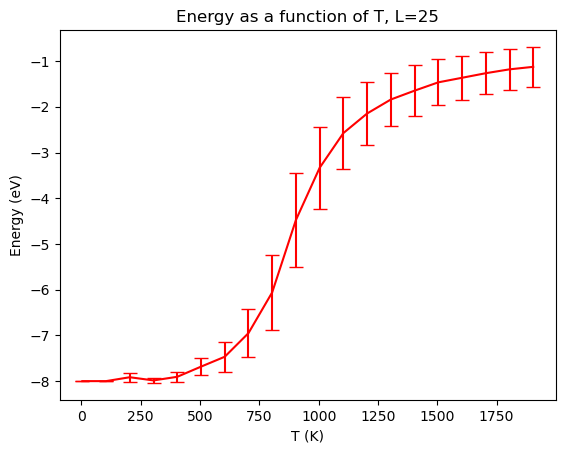
\includegraphics[width=0.7\textwidth]{images/cenergy25.png}
    \end{figure}

\end{frame}

\begin{frame}
    \frametitle{3 dimensional MC, $N=27$}

    \centering Minimum energy configuration variation with $J_0$

    \begin{figure}
        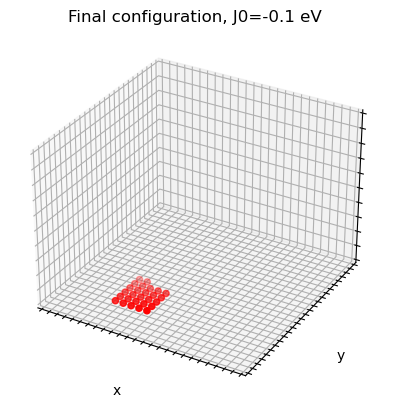
\includegraphics[width=0.7\textwidth]{images/dconf-0.1.png}
    \end{figure}

\end{frame}

\begin{frame}
    \frametitle{3 dimensional MC, $N=27$}

    \centering Minimum energy configuration variation with $J_0$

    \begin{figure}
        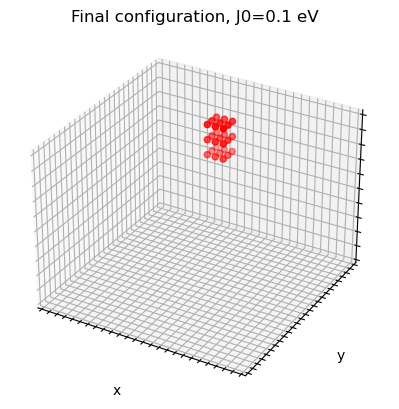
\includegraphics[width=0.7\textwidth]{images/dconf+0.1.png}
    \end{figure}

\end{frame}

\begin{frame}
    \frametitle{3 dimensional MC, $N=27$}

    $$N1/N\,@\,T=0\,K$$
    
    \begin{figure}
        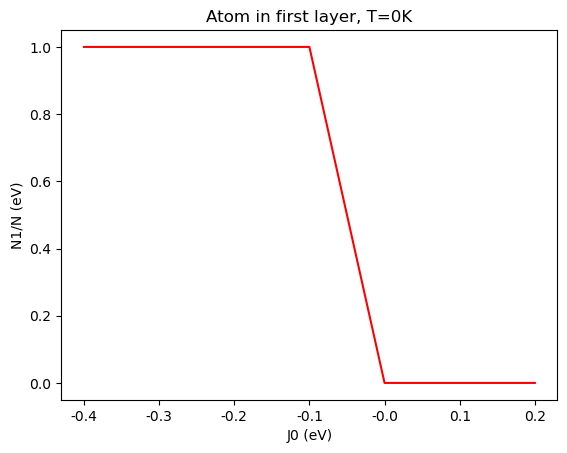
\includegraphics[width=0.7\textwidth]{images/dratio0K.png}
    \end{figure}

\end{frame}

\begin{frame}
    \frametitle{3 dimensional MC, $N=27$}

    $$N1/N\,@\, T=500\,K$$
    
    \begin{figure}
        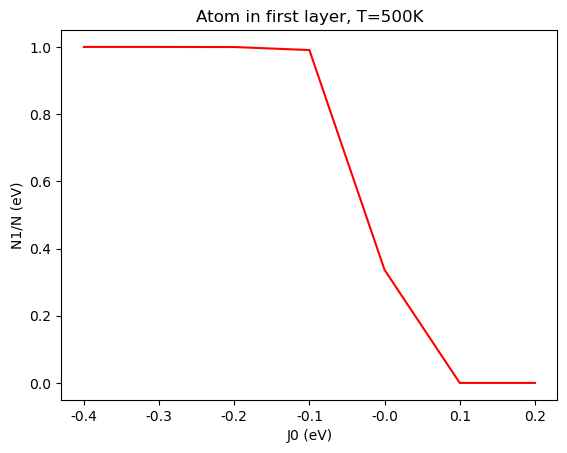
\includegraphics[width=0.7\textwidth]{images/dratio500K.png}
    \end{figure}

\end{frame}

\begin{frame}
    \frametitle{3 dimensional MC, $N=27$}

    $$N1/N \,@\, T=1000\,K$$
    
    \begin{figure}
        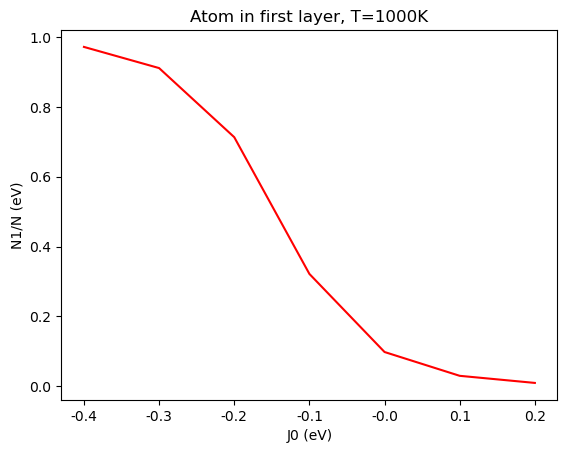
\includegraphics[width=0.7\textwidth]{images/dratio1000K.png}
    \end{figure}

\end{frame}

\begin{frame}
    \frametitle{3 dimensional MC, $N=27$}

    $$N1/N \,@\, T=1000\,K$$
    
    \begin{figure}
        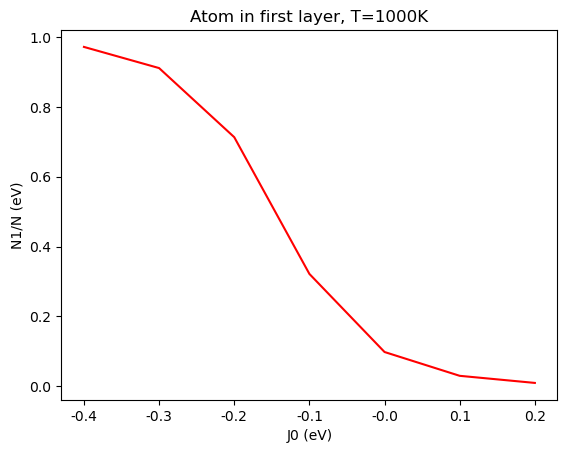
\includegraphics[width=0.7\textwidth]{images/dratio1000K.png}
    \end{figure}

\end{frame}

\begin{frame}
    \frametitle{3 dimensional MC, $N=27$}

    $$N1/N \,@\, T=1000\,K$$
    
    \begin{figure}
        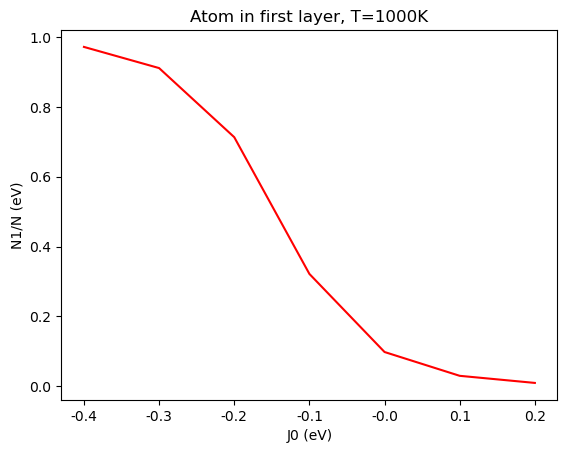
\includegraphics[width=0.7\textwidth]{images/dratio1000K.png}
    \end{figure}

\end{frame}






\end{document}